\documentclass{standalone}
\usepackage{pgfplots}
\pgfplotsset{compat=1.18}
\usepgfplotslibrary{fillbetween}
\usetikzlibrary{perspective}

\begin{document}

\definecolor{tab_blue}{HTML}{1F77B4}
\definecolor{tab_orange}{HTML}{FF7F0E}
\definecolor{tab_green}{HTML}{2CA02C}
\definecolor{tab_red}{HTML}{D62728}


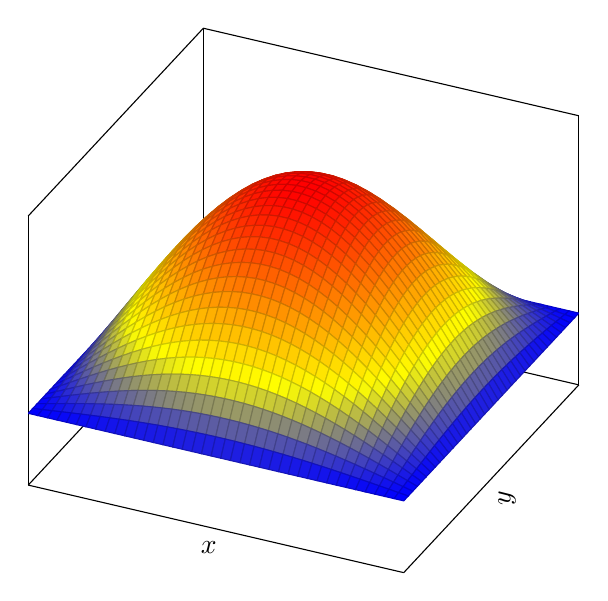
\begin{tikzpicture}[baseline]
\begin{axis}[
axis lines = box,
unit vector ratio=1 1 1,
scale=1.5, xmin=0, xmax=1, ymin=0, ymax=1, zmin = -0.2, zmax = 0.55,
ticks=none,
xlabel=$x$,
ylabel=$y$,
%zlabel=$z$,
]

\addplot3 [domain=0:1, domain y=0:1, samples=40, samples y=40, surf] {0.5*sin(deg(pi*x))*sin(deg(pi*y))};

\end{axis}
\end{tikzpicture}

\begin{tikzpicture}[baseline]
\begin{axis}[
axis lines = box,
unit vector ratio=1 1 1,
scale=1.5, xmin=0, xmax=1, ymin=0, ymax=1, zmin = -0.2, zmax = 0.55,
ticks=none,
xlabel=$x$,
ylabel=$y$,
%zlabel=$z$,
]

\addplot3 [surf] gnuplot[raw gnuplot] {
    splot 'double_integral1_data.txt' using 'x':'y':'value'
};

\end{axis}
\end{tikzpicture}

\end{document}